\chapter{Verfahrensbeschreibung}
\label{chap:Verfahrensbeschreibung}

\section{Vorgehensweise}

Nach dem Einlesen der Eingabedatei und dem Überprüfen auf Korrektheit wird, sofern das Eingabeformat nicht eingehalten worden ist, eine Ausgabedatei mit der Benachrichtigung einer falschen Eingabe erstellt. Ist hingegen das Eingabeformat eingehalten worden, startet das Spiel Nim und ein Feld mit der vorgegebenen Startverteilung wird erstellt. Solange das Spielfeld Streichhölzer enthält fordert die Kontrolle-Klasse die Spieler abwechseln auf einen Zug zu tätigen und gibt diesen anschließend aus. \newline
Zur Problemlösung eine geeignete, möglichst gute, Spielstrategie für Spieler 1 zu entwickeln wurden einige Sonderfälle betrachtet: Es gibt einige Spielsituationen die auf jeden Fall zu einem Sieg führen. Um eine gute Spielstrategie zu entwickeln ist es daher nötig eine solche Situation zu erschaffen. Ziel es dabei immer die Situation zu erhalten, immer den Gegner dazu zu zwingen ein letztes Streichholz aus der vorletzten bestehenden Reihe zu entnehmen, um selber die letzte Reihe leeren zu können.\newline
Sofern nur noch zwei Reihen existieren ist es optimal, wenn man immer so zieht, sodass die Anzahl der Streichhölzer in beiden Reihen gleich ist.\newline
Wenn die aktuelle Anzahl der belegten Reihen gleich drei ist, sollte man grundsätzlich versuchen die Spielsituation (3,2,1) zu kreieren. Gibt es die Spielsituation jedoch schon her, dass die Anzahl zweier Reihen gleich ist, so sollte die dritte Reihe komplett leer gezogen werden, da man so zu einer gewünschten Spielsituation mit zwei Reihen gelangt. Kann beides nicht erreicht werden, so gilt, dass man stets versucht die Anzahl der insgesamt liegenden Streichhölzern gerade zu halten. Diese Strategie greift auch wenn die Anzahl der Reihen größer oder gleich vier ist. Die einzige Einschränkung wäre eine Spielsituation mit vier Reihen, wenn eine Reihe ein, eine Reihe zwei und eine Reihe drei Streichhölzer enthält, da man mit dem Wegnehmen der vierten Reihe die gewünschte Spielsituation mit drei Reihen erhält.\newline
Gelangt man selbst durch das Wegnehmen einer geraden Anzahl an Streichhölzern in eine der gewünschten Situationen sollte man immer nur ein Streichholz entfernen um die Anzahl der verbliebenen Spielzüge möglichst groß zu halten, damit die Zufallsstrategie einen Fehler begehen kann.  \newline

Es folgt ein Beispiel, welches die Strategie veranschaulicht: \newline
\# Eigenes Beispiel \newline
Startverteilung: (1,2,3,4,5,6) \newline
Gewonnene Spiele Spieler 1: 100\% \newline
Gewonnene Spiele Spieler 2: 0\% \newline
Zug 1, Spieler 1: (1,2,3,4,5,6) -> (0,2,3,4,5,6) \newline
Zug 2, Spieler 2: (0,2,3,4,5,6) -> (0,2,1,4,5,6) \newline
Zug 3, Spieler 1: (0,2,1,4,5,6) -> (0,2,1,4,5,4) \newline
Zug 4, Spieler 2: (0,2,1,4,5,4) -> (0,2,1,3,5,4) \newline
Zug 5, Spieler 1: (0,2,1,3,5,4) -> (0,2,1,3,2,4) \newline
Zug 6, Spieler 2: (0,2,1,3,2,4) -> (0,2,1,3,2,1) \newline
Zug 7, Spieler 1: (0,2,1,3,2,1) -> (0,2,0,3,2,1) \newline
Zug 8, Spieler 2: (0,2,0,3,2,1) -> (0,1,0,3,2,1) \newline
Zug 9, Spieler 1: (0,1,0,3,2,1) -> (0,0,0,3,2,1) \newline
Zug 10, Spieler 2:(0,0,0,3,2,1) -> (0,0,0,2,2,1) \newline
Zug 11, Spieler 1:(0,0,0,2,2,1) -> (0,0,0,2,2,0) \newline
Zug 12, Spieler 2:(0,0,0,2,2,0) -> (0,0,0,2,1,0) \newline
Zug 13, Spieler 1:(0,0,0,2,1,0) -> (0,0,0,1,1,0) \newline
Zug 14, Spieler 2:(0,0,0,1,1,0) -> (0,0,0,1,0,0) \newline
Zug 15, Spieler 1:(0,0,0,1,0,0) -> (0,0,0,0,0,0) \newline

In den ersten vier gespielten Zügen von Spieler 1 (Zug Nr. 1,3,5,7) zieht Spieler 1 eine beliebige Anzahl Streichhölzer weg, sodass eine gerade Anzahl an Streichhölzern liegen bleibt. Im Zug 9 erkennt Spieler 1, dass mit dem Wegnehmen einer Reihe die gewünschte Spielsituation mit drei Reihen erschaffen werden kann (3,2,1). Egal wie Spieler 2 reagieren würde wird Spieler 1 nun das Spiel gewinnen, denn nun besteht immer die Chance eine gewünschte Spielsituation mit zwei Reihen zu erhalten für Spieler 1. Im 11. Zug kann er eine (2,2) Situation und im 13. Zug eine (1,1) Situation erzwingen. 


\section{Gesamtsystem}

\subsection{Main-Funktion}
Die Main-Funktion erzeugt den Controller IControl. An diesen wird der Dateipfad weitergegeben. Das Spielgeschehen erfolgt nun in IControl.

\subsection{Model}
Hier sind die wesentlichen Klassen, die die Spieldaten und Algorithmen enthalten und auf ihnen operieren. Es ist kein expliziter Zugriff auf die Daten möglich, lediglich über die Schnittstelle IControl kann auf diesen zugegriffen werden. Zum Model gehören die zwei Interfaces IModel, welches die Spielinfos enthält, und IAlgo, welches die beiden Spielstrategien für Spieler 1 und Spieler 2 enthält.


\subsection{View}
Die Ein-/Ausgabe wird in der View vorgenommen. Dazu besteht für Input und Output jeweils ein vorgegebenes Eingabe- und Ausgabeformat. Beim Einlesen der Daten soll dabei schon auf Korrektheit überprüft werden.

\subsection{Controller}
Im Controller werden die Daten über die View in das Model eingelesen. Mithilfe der Spielinformationen vom Model kann der Controller das Spiel leiten.

\newpage

\section{Datenfluss}
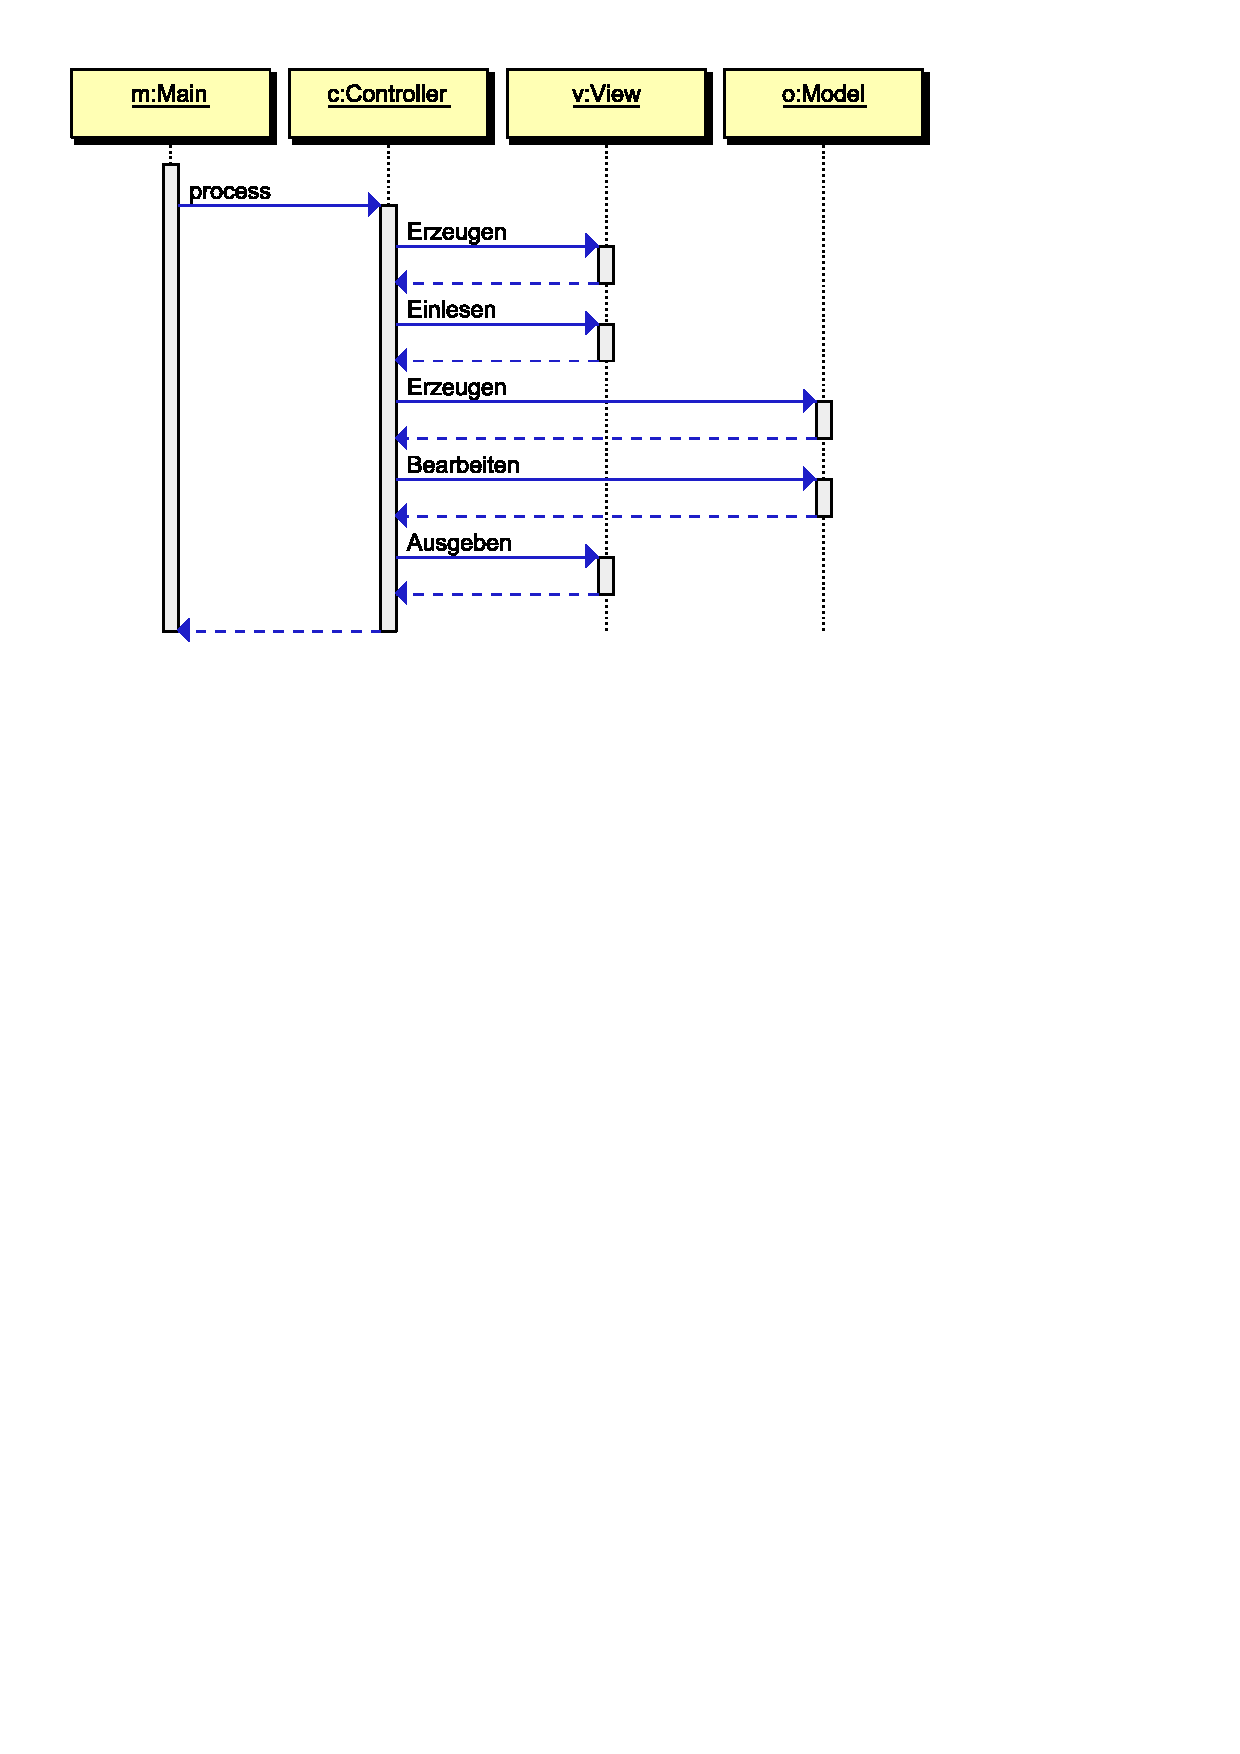
\includegraphics{Diagramme/sequenz2.pdf}